%\documentclass[12pt,a4paper,titlepage]{article}
%\documentclass[12pt]{report}
\documentclass[12pt, a4paper,titlepage]{extreport}
\usepackage[utf8]{inputenc}
\usepackage[english]{babel}
\usepackage{amsmath}
\usepackage{amsfonts}
\usepackage{amssymb}
\usepackage{makeidx}
\usepackage{graphicx}
\usepackage[font=small,labelfont=bf]{caption} % Required for specifying captions to tables and figures
\usepackage{lmodern}
\usepackage{kpfonts}
\usepackage{titling}
% no indent after line break
\setlength\parindent{0pt}
\setlength\parskip{\medskipamount}
%\renewcommand{\familydefault}{\sfdefault}
\usepackage[default]{lato}
\usepackage[T1]{fontenc}
\usepackage{url}
\usepackage{hyperref}
\setcounter{secnumdepth}{3} 
\setcounter{chapter}{1}
%\usepackage{fontspec}
%\setmainfont[Ligatures=TeX]{Hoefler Text}
%\setsansfont[Scale=MatchLowercase,Ligatures=TeX]{Gill Sans}
%\setmonofont[Scale=MatchLowercase]{Andale Mono}
\usepackage[left=2.5cm, right=2.5cm,top=2cm,bottom=2cm]{geometry}
%\author{Francesco Gadaleta, PhD}
\date{}
\pretitle{%
  \begin{center}
  \LARGE
  \includegraphics[width=2cm,scale=1,keepaspectratio]{{fitchain_logo_dark_small.png}}\\[\bigskipamount]
}
\posttitle{\end{center}}

\begin{document}

%\begin{figure}[!h]
%   \begin{center}
%     {
\includegraphics[scale=1,width=3cm,keepaspectratio]{fitchain_logo_dark_small.png}}
%    \end{center}
% \end{figure} 
 
\title{\textbf{Amethix - fitchain}\\ The decentralized machine learning factory\\
\small{TECHNICAL PRIMER}}
%\title{fitchain.io\\ The machine learning platform to analyse data \\with confidentiality in mind }

\author{\textit{Francesco Gadaleta, Ph.D.}\\ \textit{Daan Gerits}}
\maketitle


\begin{abstract}
This paper provides an introduction to the \textbf{fitchain} platform. 

The fitchain platform allows data providers to open their private data to algorithms created by data scientists while maintaining secrecy and confidentiality. Three major actors are involved in the process of sharing data and training machine learning models: \textit{model owners} (usually data scientists) who provide the model source code, \textit{data owners} (usually organisations) who provide the data to train machine learning models on and \textit{model verifiers} who validate the models after they have been trained and provide evidence to model owners' claims.
 
The protocol implemented by \textit{fitchain} prevents potentially malicious code submitted by \textit{model owners} from tampering with the private infrastructure of \textit{data owners}. In addition, \textit{fitchain} guarantees that the source code submitted by \textit{model owners} is executed as is. \\
In light of these two essential requirements, the fitchain platform can accommodate the needs of organisations to let their private data be analysed by leveraging a global pool of data scientists who want to provide solutions to the machine learning problems at hand, in exchange of appropriate incentive. When security and confidentiality are preserved across the entire process, both data and models become valuable assets that can be traded in the data-model marketplace. 
A reward assigned to each project, together with the additional incentives for model validators will keep the fitchain marketplace sustainable and balanced, around what we have identified as a Nash equilibrium \cite{nash}.
\end{abstract}

\section{Introduction}
In the era of machine learning, characterised by more and more powerful hardware. more accurate predictive models, and the capability to collect large amounts of data, both organisations and individuals feel the urge to act on their data as they never did before, in order to extract some sort of value that would be beneficial to their business. The progress of machine learning \footnote{Gartner Says AI Technologies Will Be in Almost Every New Software Product by 2020, \url{https://www.gartner.com/newsroom/id/3763265}} and the success achieved in transforming raw data into knowledge is undeniable \footnote{2018 AI predictions 8 insights to shape business strategy, \url{https://www.pwc.com/us/en/advisory-services/assets/ai-predictions-2018-report.pdf} } 

Data driven decisions are essential for organisations with complex business dynamics, in which human intervention is usually less effective, often prone to error, and generally speaking much slower than the pace of collecting the data itself. As a matter of fact, data has become a valuable asset, sometimes more valuable than traditional ones. Not only for IT giants like Google, Facebook and Twitter, but also for pharmaceutical and financial corporations it is essential to act on data in order to maintain an advantageous position with their competitors and take decisions faster, minimising losses and maximising profits. As a consequence, the figure of the data scientist has acquired a fundamental role within the settings of many data-driven organisations.

In light of these undeniable facts, no organisation can ignore what we have identified during the years. Data scientists

\begin{itemize}
\item define the quality of the final result of their models
\item prefer to work on challenging problems
\item can not always get access to the data they need
\end{itemize}

Highly skilled data scientists are more likely to design and implement higher predictive models. Hence, hiring the best data scientists in the market can be a game changer for competitive organisations. In addition, initiatives like \textit{Kaggle} \cite{kaggle} confirm the fact that highly skilled data scientists prefer to work on challenging problems and they have the tendency to change application domain, in order to explore new opportunities and put their models to new tests.
Finally and more importantly, regardless of the domain, it is very difficult to get access to insightful and high quality data, if not after signing non-disclosure agreements (NDAs), or other forms of collaboration contracts that protect secrecy and confidentiality about the data to be shared and the business processes involved.

In contrast, organisations are experiencing other limitations, namely they

\begin{itemize}
\item can not always share their data due to size (that keeps increasing) or due to governance restrictions
\item can not keep highly skilled data scientists for very long periods in their teams
\item can not always act on private data that, in turn, keeps getting outdated 
\end{itemize}

The main challenge addressed by \textit{fitchain} consists in allowing data scientists  design their models on data they cannot access, or equivalently to grant organisations access to a global pool of data scientists without sharing any confidential information with them. 
This is not an easy task for the reasons we identify in the following paragraphs. 


\paragraph{Security}
If data cannot be transferred outside the organisation's infrastructure, then models should be transferred and trained at the organisation's site. This clearly opens the doors to a plethora of attacks that can be triggered by malicious code, hidden behind a legit machine learning model, tampering with the organisation's infrastructure during model training

\paragraph{Non-repudiation}
Any model that is submitted by a data scientist must be executed \textit{as is}, without the organisation to interfere with the data scientist's implementation and decisions. This requirement usually collides with the security issues that might arise as explained in the paragraph above

\paragraph{Traceability}
Any model that has been trained at the organisation's site, must be traced and uniquely identified before it is deployed or integrated within a business context. Moreover, as any other valuable asset, models can be traded and utilised by other organisations and data scientists. Traceability and reputation are two essential requirements for any software service that is built with the effort of multiple peers, spread in different geographical locations.

We have designed the \textbf{fitchain} platform to accommodate the aforementioned objectives. 


\section{The Fitchain Ecosystem}\label{ecosystem}
Organisations that want to leverage machine learning to extract insight from their private data and extract value for their business, have very few options than undergoing the long process of hiring talented data scientists in a market that is becoming more and more polluted and noisy\footnote{How to Consistently Hire Remarkable Data Scientists, \url{http://firstround.com/review/how-to-consistently-hire-remarkable-data-scientists}}. 
With fitchain the traditional process of acquiring human resources with special skills will radically change, allowing organisations to interact with data scientists on a per-project basis. For the sake of explaining the plausible processes within the fitchain ecosystem, we hereby identify three actors: the data provider, the model provider and  the model validator.

\subsection{The Data Provider}

\begin{center}
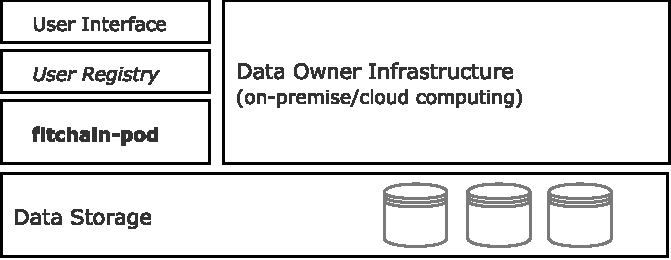
\includegraphics[scale=1]{pod_dataowner.pdf} 
\captionof{figure}{Architecture of the fitchain-pod integrated with the Data Provider's infrastructure. The fitchain-pod orchestrates requests to use private data from other actors legitimately registered to the User Registry}
\end{center}

The organisation that own private data and need to solve a machine learning problem, will connect to the \textbf{fitchain} platform as \emph{Data Provider}, in order to submit a description of the problem to be solved, together with a template of the data required by a data scientist. 
The aforementioned template is generated by the \textbf{fitchain-pod}, a component that is executed locally within the organisation's infrastructure and that is directly connected to the data. The pod is managed via a user friendly interface running in the local browser of the data provider.
 
The data template is \textit{not} the original data and \textbf{does not} contain any sensitive information that would allow anyone to reconstruct the original data source. This is an essential requirement for any organisation to submit their projects publicly and expose only a picture of their data (the original data must remain private).
The owner of the project (eg. the data provider, or any other actor in the fitchain ecosystem) can allocate a project reward that will incentivise data scientists to provide viable solutions for. More specifically, such a reward is the currency that will be used to remunerate the data scientists who provide the best solution, together with the actor who provides the infrastructure for training and the validators who assess the accuracy of the model (as described in the next paragraphs).
Once a model has been submitted, the \textit{fitchain-pod} executed by the data provider, orchestrates and controls the process of model training, during which traces are generated and stored permanently to the available blockchain-based ledger.
The original data source is never modified nor shared in any form. As this is the only location where data is available, enforcing global and local regulations (even for the most recent General Data Protection Regulation (GDPR) enforced by EU \cite{GDPR}) becomes a straightforward task.

\subsection{The Model Provider}

\begin{center}
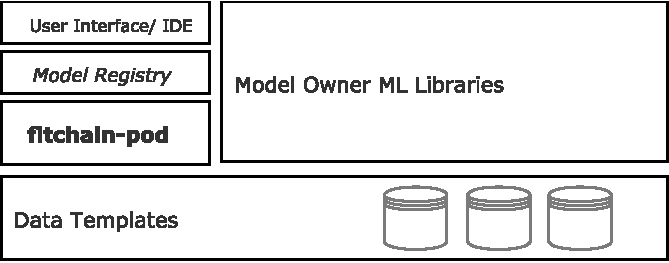
\includegraphics[scale=1]{pod_modelowner.pdf} 
\captionof{figure}{Architecture of the fitchain-pod at the Model Owner's side. This is where the model is implemented with the aid of data template, provided by the data owner's pod. The fitchain pod orchestrates submissions and remote execution of models, tracing them on the Model Registry.}
\end{center}

Data scientists who want to develop a predictive model in the domain of interest can connect to the fitchain platform as \emph{Model Provider}. Such a data scientist might be looking for submitted projects in search for a solution. Needless to say,\emph{Model Provider} will choose the project that is more convenient to her in terms of effort, required skills and offered reward, after which she will start working on a model implementation. This would be possible due to the fact that the project description is supplied with the data template that can be used to assess the compatibility of the model with the original data. A model that \textit{works} on the data template, is supposed to work on the original data too (provided the data owner is not changing the original data without informing her \textit{fitchain-pod}).
Once a model has been implemented and submitted, the pods of the actors involved in the process will orchestrate model deployment and model training within the organisation's infrastructure, the only location where the real (private) data is stored and made available. 

\subsection{The Model Validator}
Any model that is remotely trained, requires to be validated, in order to be deployed in production environments. As a matter of fact, a malicious organisation could train models on fake data, or could fake the entire model training process. 
Model validation is an essential task that is twofold: it discourages organisations to fake model training and assesses the predictive power of models as they become available assets within the fitchain ecosystem.
The model validation process consists of a set of interactions between two actors: \textit{the prover} and \textit{the verifier}. The protocol implemented to validate models by consensus has been designed as an interactive zero-knowledge\cite{zxsnarks} proof system, the details of which will be reported in the \textit{fitchain whitepaper} (coming soon).

The two actors of the model validation process are 

\paragraph{Prover}  The entity who trained the model and claims its capabilities and metrics (eg. accuracy, error rate, false positive/negative rate, etc.) over the training data

\paragraph{Verifier}  The entity who verifies that the aforementioned claims about the model are consistent. Namely, a verifier can create or use validation data of which the response is known, in order to assess the claimed accuracy of the model on such data

In order to perform verification, both validation data and model metrics - which together are referred to as \textit{the challenge} - must be accessible at any point in time. Therefore they are stored onto the fitchain public registry. We identified technologies like \cite{oceanprotocol}, BigchainDB \cite{bigchaindb} and IPFS \cite{ipfs} to annotate and trace the validation datasets that are used for model verification.
Technically speaking the challenge-based model verification process is equivalent to the block mining process for blockchains like Bitcoin \cite{bitcoin} and Ethereum \cite{ethereum}.
 
Together with the traces generated by the pod during training, the model verification process constitutes what we refer to as the \textit{proof-of-train}. 
Needless to say, no sensitive data is stored to the public ledger, nor transferred anywhere else, as the sole purpose of the \textit{proof-of-train} mechanism consists in guaranteeing that organisations and data scientists do not violate the security requirements of the fitchain platform.


\section{Use Cases}
The fitchain platform has been designed to accommodate the needs of highly regulated environments in which data confidentiality and industrial secrecy must stay protected, while giving the opportunity to external actors to interact and use private data. While the most common scenarios would be represented by organisations who own large or diverse data sets and fewer resources to analyse them, the \textit{fitchain pod} would also accommodate the needs of individuals who want to  monetise their data by allowing other actors to use it without accessing or ever own it. 

Among the numerous scenarios in which data analytics has already proved to be effective, healthcare is the one we believe will have higher impact on society, as soon as solutions to unlock sensitive data are found. 


\subsection{Healthcare\&Pharma}
The primary mission of fitchain is to unlock the value of highly sensitive data, owned by pharmaceutical and healthcare institutions. As a matter of fact, healthcare and pharmaceutical institutions represent one of the most regulated environments in data science. Pharmacological and medical data, chemical compounds in the field of drug discovery, medical claims for real-world evidence (RWE), and sales statistics of drugs in companies' portfolios, represent only a tiny fraction of the amount of data that such organisations usually store in their infrastructures and deal with.

We strongly believe our mission is going to impact research and development as well as bring social benefit on a global scale.  
Acting on such data via machine learning and predictive analytics is one powerful strategy that many organisations have already experienced and cannot deny its benefits. Entire organisations have been restructured to weaponise themselves with teams of data scientists in order to extract hidden knowledge from their data, otherwise sitting in their infrastructure, becoming obsolete and more expensive to store. 
The pool of available data scientists however is not unlimited and the scarcity of such skilled individuals has led the very same organisations to deal with external contractors, or to hire the data experts the local market had to offer. 

It is one goal of fitchain to facilitate the way data scientists interact with organisations. We believe in a world in which healthcare and pharmaceutical organisations interact with their collaborators, globally spread, without any constraint. Bridging the gap between private data and data scientists on a global scale is a fundamental step that allows large and small healthcare institutions to cooperate with data experts otherwise not accessible. This will, in turn, provide the best solutions to the problems submitted via the fitchain platform.

There are very common scenarios in which trans-institutional curated data is mostly required for advanced medical research and analytics. More specifically, precision medicine utilises genomics and traditional clinical data to assess risk to disease. Clinical trials depend on unstructured and interconnected data, usually stored in different silos. In such complex contexts, it is important to consume data wherever it is created or collected, without the necessity to move it across cloud storage facilities. This facilitates the process of analytics because the risk of data leakage and loss are dramatically reduced. 

Fitchain brings computing to the data, facilitating the training of machine learning models, and redistributing the aforementioned trained models from their owners to their direct users, achieving far greater levels of insight in medical data.

\subsection{Finance and Banking}
Banks and financial institutions represent another highly regulated environment that has never experienced shortage of data. From financial transactions of individuals, to insurance claims and trading ticks, the amount of data in the financial sector is growing at a very fast pace and does not seem to slow down any time soon. 
Financial institutions have realised the importance of machine learning models for their business, to the point that many of them have clearly switched the typology of their business from financial companies to data companies \footnote{Financial Services,  \url{https://www.infosys.com/data-analytics/verticals}}. 

The data science task force required to transform raw data into knowledge usually demands a very time consuming process to guarantee that sensitive information never leaves the organisation's headquarters. Data encryption, de-identification and data randomisation, or simply legal contracts and NDAs (Non Disclosure Agreements) are only a few strategies to share private data outside the organisation. However, it is not always feasible to guarantee the strict requirements of data protection. In many such cases, episodes of insider trading or competitor advantage have characterised and compromised the business of the affected organisations.

A platform like fitchain will allow a global pool of incentivised data scientists to operate the sensitive financial data of organisations without exposing it to the public. With the fitchain platform, such data scientists will be rewarded proportionally to the accuracy of the solutions they provide, pretty much the same way as on a Kaggle \cite{kaggle} competition. This time without publishing any data.


\subsection{Personal Data}
Fitchain will also work for individuals who own the data they produce. Unfortunately, it is uncommon to think that people own the data generated by their mobile devices, their browsers, their keyboards, the electricity meters of their houses, and any digital device at their disposal. 
Organisations like Google, Facebook, Amazon, and Twitter have built empires on top of data they do not legally own.

With fitchain, individuals will have a tool to claim their data and monetise it. As any other asset, data can be traded, or rented to whoever needs it to train machine learning models. 
It is legitimate to think that the same organisations that today profit from individuals' data will train their models, by paying a price defined by the market or the users themselves.

As a matter of fact, everyone can open their data to the public without disclosing personal information. 
In such a scenario, fitchain fills the gap between individuals who provide the data and organisations (or other individuals) who provide the models, via a platform that implements the data-model marketplace. 

\subsection{Research and Development}
In several domains, research is conducted by publishing results from methods (usually machine learning models) performed under specific conditions and datasets. Any claimed result requires verification and, more importantly, \textit{reproducibility}. 
Reproducible results are extremely important in order to adopt machine learning techniques and solutions that are mainly data driven. 

While deep learning and advanced machine learning methods provide very accurate predictions in domains like computer vision, medical imaging and genomics, they still depend on the training data and on a excessively high number of parameters. 

It is difficult - if not impossible - to reproduce the results of data driven solutions when data are private and cannot be shared with the public \footnote{What Are Best Practices For Collaboration Between Data Scientists? \url{https://www.forbes.com/sites/quora/2017/04/04/what-are-best-practices-for-collaboration-between-data-scientists/\#7b448eb8335e} }. 
As a consequence, non reproducible models are difficult - if not impossible - to deploy in production environments. Hence, claims that cannot be verified will slow down the pace of innovation and the adoption of novel analytical strategies, even when it is evident how such results improve the state of the art.

With fitchain, researchers can leverage the capabilities of remote computations on private data. This, in turn increases reproducibility required to validate such novel techniques.
Fitchain provides a way to perform interactive challenges, to validate machine learning models that have been trained on private data. Traceable and reproducible results are several steps closer to wide stream adoption. 

\section{Architecture}
In order to operate in the fitchain platform, the actors described in Section \ref{ecosystem}, are required to expose the schema of private data to a global (or local) community of data scientists who will, in turn, submit their solutions in the form of machine learning models. Submitting the schema is a task performed by data owners, while submitting machine learning models is a task performed by model owners. 
It is possible for an actor to play the role of data owner for a project and model owner for another (\textit{symmetric} fitchain-pod).

Both data owners and model owners execute a gateway application, referred to as the \textit{fitchain-pod}. The \textit{pod} is the essential software component that orchestrates processes in the fitchain marketplace.
The team at fitchain have engineered such a critical component in order to facilitate the integration within diverse execution environments, such as public/private/hybrid cloud and on premise. 
Organisations that perform their analytic pipelines in any of the aforementioned environments are ready to execute the fitchain-pod and start sharing their data or their models. 

\subsection{Infrastructure Requirements}
While the requirements of the pod can differ according to the specific use case, it is in the organisation's responsibility to allocate a sufficient amount of resources to accommodate the execution of a number of models and specific amount of private data.

Data owners who have access to private computing resources and storage, will allocate such resources as part of the \textit{fitchain grid}. The pod will connect models to the data stored in the private storage and will orchestrate model training across the allocated computing units. 

Equivalently, data owners who have access to resources in their Virtual Private Cloud such as those provided by Amazon AWS, Microsoft Azure and Google Cloud, can connect a \textit{fitchain pod} to orchestrate model training in the cloud. Private data can be connected to the pod in similar fashion, regardless of the type of storage, local or remote.
  
\section{The Marketplace}
A platform that matches the needs of organisations to the skills of data scientists can exist only if all the actors involved in the process are rewarded as soon as they perform their tasks. In any blockchain ecosystem, the actors who perform maintenance of the chain and prevent fraudulent scenarios like double spending and inconsistency of account balances, are rewarded with cryptocurrency (as for Bitcoin and Ethereum miners). 
In the fitchain marketplace every actor that plays a role can be rewarded too. Specifically

\begin{enumerate}
\item organisations will have their data science problems solved
\item the data scientists who solved the problem will gain the project reward allocated by the organisation
\item model validators will gain their reward for checking if the model has been correctly trained
\item trained models that are used by other peers will generate revenue
\end{enumerate}

In such a marketplace, it is essential that every entity is considered an actor and is attributed a \textit{reputation score} that is always visible to the other actors. 
An organisation who never completed model training, a data scientist who attempted to tamper with private infrastructure or who never achieved acceptable accuracy with her models, a miner who did not contribute to consensus, a machine learning model that was not performing as claimed during model training, are all examples of actors with low reputation.

The reputation score is built as all the actors keep interacting in the marketplace. Therefore it is a dynamic and adaptive score that reflects the state of the network and all interactions thus far, similarly to financial wallets of a bank or a blockchain. 
Details about how such a reputation score is calculated will be provided in the whitepaper.


\pagebreak 
\section{Security Concerns}
A system that facilitate the interaction between non authenticated peers and private assets must be considered critical, when it comes to security concerns. In this section we expand on the three most critical security issues that might arise by such interaction and should be addressed in order to guarantee protection for the private assets an organisation decided to unlock. The first concern regards infrastructure and data escapes. The second security issue is about escaping data via machine learning models while the last concern is about faking the training process.

\subsection{Concern 1: Infrastructure Security and Data Escapes}
Executing code that has been created by non authenticated peers is, without any doubt a major concern for the organisation that is executing such code. 
As a matter of fact, a malicious data scientist might write code that attempts to attack the organisation's infrastructure internally in order to leak industrial secrets, steal employees identities and other assets.

The fitchain pod implements security mechanisms to prevent the aforementioned types of attack. In fact, submitted code is executed in a completely isolated environment, that has no direct access to the private data sources, nor to the network and the rest of the infrastructure.

The purpose of such a strong isolation layer is twofold as 1) it prevents malicious code from tampering with the organisation's facilities and 2) it prevents private data to be accessed by entities other than those that have been granted access.


\subsection{Concern 2: Machine Learning Model Escapes}
Another typical attack that is possible on \textit{any} platform that allows code - and more specifically machine learning models - to be trained remotely, is referred to as \textit{model escape attack}. 
Without loss of generality, a machine learning model is a complex mathematical function that calculates an \textit{output} given an \textit{input}. What makes such a input-output association possible is a set of numbers, usually referred to as \textit{model parameters}, that are tuned during so called model training phase. 
The complexity of a model is directly proportional to the amount of model parameters that are trained. For instance, in the relatively simple linear regression model in Equation \ref{linregr}

 \begin{equation}\label{linregr}
 y=\beta_0+\beta_1 x_1 + \beta_2 x_1^2 + \beta_3 d_1 + \beta_4 d_2 + \beta_5 d_1 x_1+ \beta_6 d_2 x_1  
 \end{equation}
 
there are $7$ parameters to be trained from the data \footnote{This includes the main effect, quadratic effects, interaction effects and the intercept}
 
A 5-layer convolutional neural network \cite{CNN} with the layer dimensions reported below

\textit{
input ($28x28$), convolution\_1 $32x(5x5)$, \\
maxpool\_1 $(2x2)$, \\
convolution\_2 $32x(3x3)$, \\
maxpool\_2 $(2x2)$, \\
fully\_connected $(256x1)$, \\ 
output $(10x1)$ } \\

has $217706$ trainable parameters. 

It is, however, very common to train more complex neural networks with $300M$ parameters or more. 

A malicious data scientist can rely on such a high number of parameters as a viable mean to carry private data outside the organisation. This could be achieved even by training a machine learning model that implements the so called \textit{identity function}, a mathematical function that can identically map the input to the model parameters. This would, in turn, legitimately carry private data outside the data owner's infrastructure, in the form of model parameters. 

Fitchain prevents such scenarios from happening, by solely communicating machine learning metrics (not model parameters) to the data scientist. Model parameters will be encrypted whenever the model is exported outside the organisation. Technical details about such a methodology will be provided in the whitepaper.

\subsection{Concern 3: Fake Model Training}
A malicious organisation have several options to fake model training. Changing the schema of the training set right after a model has been submitted from a data scientist, or changing the data directly (and keeping the same schema) right before training a model, are only a few strategies to create models that perform with erroneous accuracy.

While model validators can still detect that the claimed accuracy for a fake model does not hold during the validation phase, it would be extremely beneficial to detect such scenarios immediately. 

Fitchain implements a complex signalling mechanism to generate blockchain transaction logs during all the phases of interaction. Transaction logs are created  

\begin{itemize}
\item when private data are connected to a project
\item whenever a model is submitted
\item when private data are connected to the model 
\item during model training 
\end{itemize}

Tracking all the phases of an interaction between any two actors provides high security guarantees about the authenticity of the model. External actors are always capable of inspecting and validating the state of the interaction during and after model training.


\pagebreak
\section{Conclusion}
It is undeniable that data scientists allow organisations to venture into machine learning and experience the numerous potential benefits of predictive models. An essential requirement for organisations is to make their data accessible to the data scientists who will operate and train their models. Such access is usually granted via legal contracts and non disclosure agreements and the usual long and tedious hiring process. 

With fitchain, organisations can unlock the value of their data instantly, connecting them to a global pool of data scientists to effectively work on a solution and train their models. As no data is shared, except for an initial schema and a problem description, no addition confidential information is expected to leave the organisation, who can keep their industrial secrets and data private.

The security mechanisms that are implemented in the \textit{fitchain-pod} provide guarantees for both the organisation and the data scientist. A blockchain component connects the dots and keeps the registries of all the actors involved in the process, providing a tamper-free reputation-based mechanism for data owners, model owners, miners and trained models.

Data, machine learning skills and models are tradeable assets in the fitchain marketplace, defined as the decentralised, secure and traceable machine learning factory.


\bibliographystyle{plain}
\bibliography{fitchain.bib}

\end{document}
